\documentclass[platex]{beamer}
\usepackage{luatexja-preset}                % LuaLaTeX する
\usepackage[zerostyle=b]{newtxtt}           % typewriter 体
\usepackage{url}
\usepackage{graphicx}
\setbeamertemplate{navigation symbols}{}    % 右下のアイコンを消す
\renewcommand{\kanjifamilydefault}{\gtdefault} % 本文ゴシック体

% タイトルの設定
\title{\textbf{WORD編集部のご案内}}
\author{WORD編集部\\\url{https://www.word-ac.net/}, \href{https://twitter.com/word\_tsukuba}{@word\_tsukuba}}
\date{2022年8月11日}   % <-- その年のオーキャンの日付にする
\begin{document}
\maketitle
\begin{frame}[plain]{「WORD編集部」って何?}
\begin{itemize}
 \item \alert{\textbf{情報科学類誌『WORD』(読み:わーど)}}の編集・発行を行う団体
 \item 情報科学類公認
 \item 記事の執筆から編集・印刷まで,すべて学生が自主的に行っている
\end{itemize}
\end{frame}
\begin{frame}[plain]{情報科学類誌『WORD』って?}
 \begin{itemize}
  \item 情報科学類生が中心となって,不定期に発行している雑誌
  \begin{itemize}
   \item 執筆者は情報科学類生に限らない
   \item 内容もコンピュータサイエンスに限らない
  \end{itemize}
  \item 年数回+特別号を発行
  \begin{itemize}
   \item 特別号の例:引っ越し準備号,入学祝い号,研究室紹介号
  \end{itemize}
  \item \alert{この類の雑誌で,現在発行しているものの中では,\\\textbf{筑波大学で最も伝統ある学類誌}}
  \begin{itemize}
   \item Since 1979(cf. 情報学類設置は1977年)
   \item 詳細は『WORD』51号\footnote{\url{https://www.word-ac.net/post/2022/0605-word51/}}をチェック!
  \end{itemize}
 \end{itemize}
\end{frame}
\begin{frame}[plain]{表紙}
 \begin{figure}
  \centering
  \includegraphics[width=32mm]{img/lab2021.pdf}
  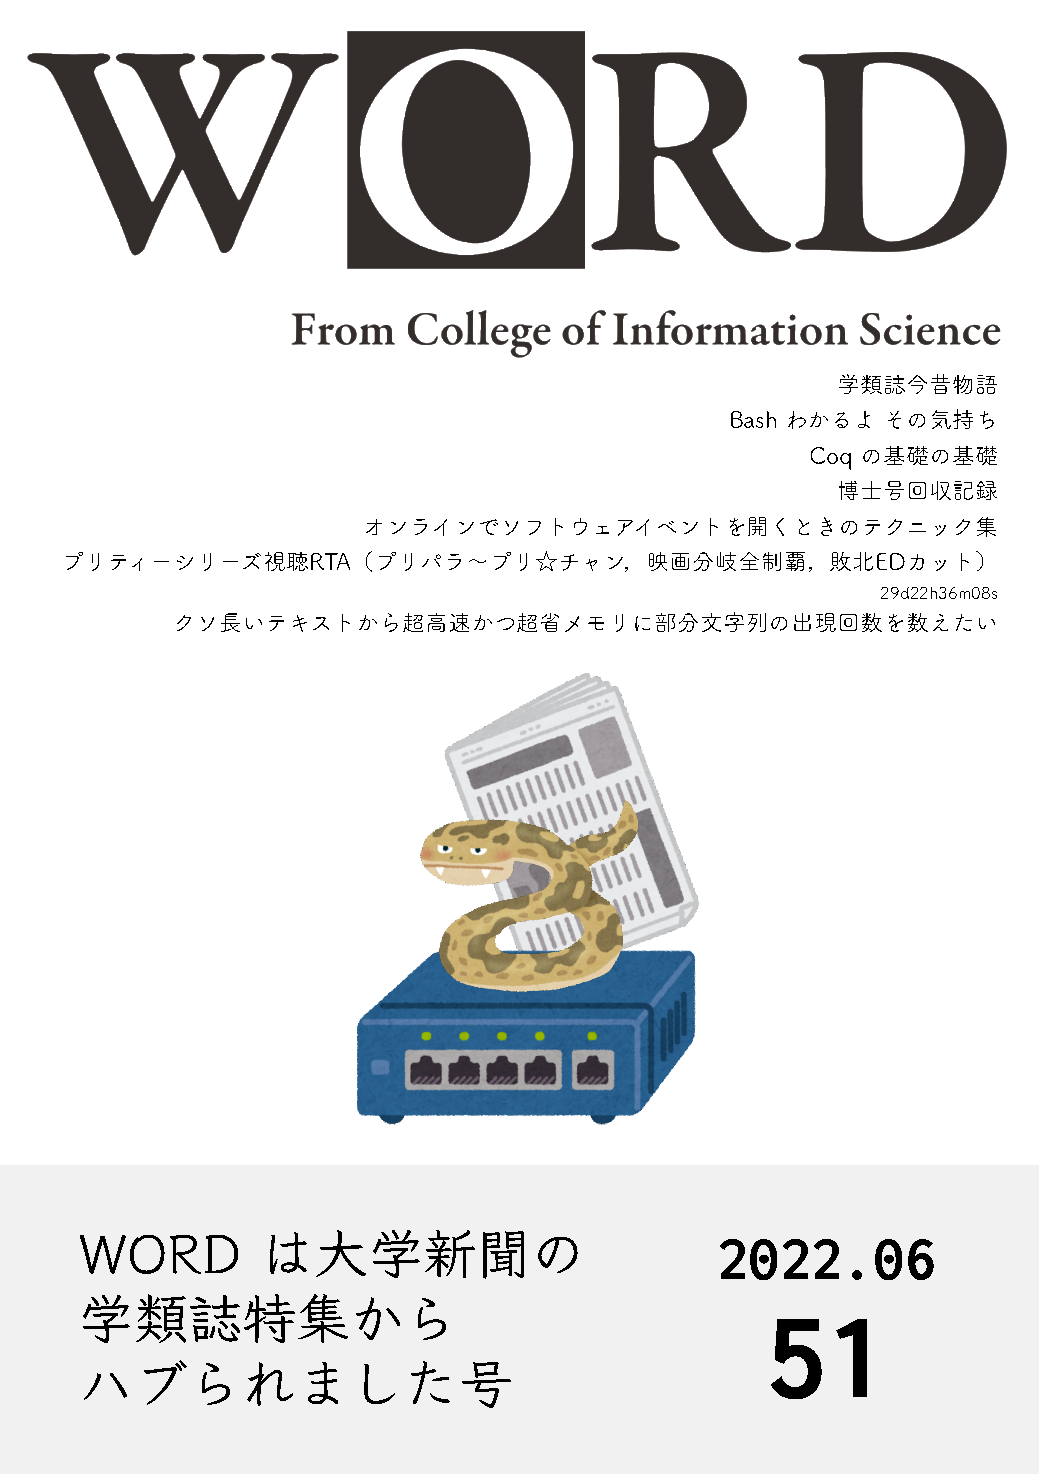
\includegraphics[width=32mm]{img/word51.pdf}
  
\includegraphics[width=32mm]{img/word52.pdf}
 \end{figure}
\end{frame}
\begin{frame}[plain]{『WORD』配布中!}
 普段は3A・3C棟で配布していますが,
\begin{itemize}
 \item 「WORDは大学新聞の学類誌特集からハブられました号」(2022/6発行)
 \item 「WORDは発行から90日経過しても読めます号」(2022/8発行)
\end{itemize}
を\alert{オープンキャンパス(物理)会場でも配布}(先着順)しています.

オープンキャンパスの記念に是非1部ずつお持ち帰りください!

※在庫切れの場合はご容赦ください.
\end{frame}
\begin{frame}[plain]{WORD編集部室(3C212)}
 \begin{itemize}
  \item 技術書の詰まった本棚
  \item 高速なインターネット環境とたくさんのパソコン・サーバ
  \item 24時間利用可能!
 \end{itemize}
\begin{figure}
 \centering
 \includegraphics[width=50mm]{img/monitor.jpg}
 \includegraphics[width=50mm]{img/hondana.jpg}
\end{figure}
\end{frame}
\begin{frame}[plain]{こんな人がいます}
 \begin{itemize}
  \item ネットワークやサーバに興味のある人
  \item (\LaTeX などの)組版に興味のある人
  \item 記事を書きたい人
  \item 自宅通学予定の人で学内に居場所が欲しい人
 \end{itemize}
\end{frame}
\begin{frame}[plain]
 \begin{center}
  \Huge\textbf{WORD編集部は,\\皆様をお待ちして\\おります!}
 \end{center}
\end{frame}
\begin{frame}[plain]{WORDから見た情報科学類の魅力}
\pause
 \begin{center}
  \Huge \alert{\textbf{学生の自主性を\\大事にしてくれる!}}
 \end{center}
\pause
WORDでの実例:
\begin{itemize}
 \item 部屋やネットワーク・サーバーの管理
 \item 記事のネタ探しや執筆
\end{itemize}
などなど,学生の自由にさせてくれるので,やりたいことが(常識の範囲内で)自由にできる!
\end{frame}
\begin{frame}[plain]{リンク集}
 \begin{itemize}
  \item \url{https://www.word-ac.net/}
  \begin{itemize}
   \item 最近の過去号はここから見られる
   \item \url{gemini://gemini.word-ac.net/}もあるよ
  \end{itemize}
  \item \url{https://twitter.com/word\_tsukuba}
  \begin{itemize}
   \item 動いたり動かなかったりするTwitter
   \item DMは開いてます
  \end{itemize}
  \item \url{https://github.com/WORD-COINS}
  \begin{itemize}
   \item issueやPRなど歓迎
   \item このスライドもGitHubで管理しています\footnote{\url{https://github.com/WORD-COINS/opencampus-slide}}
  \end{itemize}
 \end{itemize}
\end{frame}
\begin{frame}[plain]
 \begin{center}
  質疑応答
 \end{center}
\end{frame}
\end{document}